Hoy en día existe un problema que concierne  las  centrales nucleares de fisión, central termoeléctrica,  experimento de física de partículas, etc., e, incluso, en futuras centrales de fusión nuclear y es la creación de altos niveles de radiactividad en estos sitios. Por ejemplo, una central nuclear operando en modo normal puede llegar a emitir alrededor de $300\ \tera\becquerel/\giga\watt\mathrm{y}$ ~\cite{300TBq}.  Debido a la peligrosidad que ello implica estos deben ser controlados y disminuidos en la medida de lo posible.

En concreto, uno de los elementos radiactivos más abundantes generados en estos lugares es el tritio. Debido a las elevadas tasas de radiactividad anteriormente mencionada,es fundamental controlarlo en estas zonas de trabajo para evitar que contribuya a esta cifra ya que un mayor número de emisiónes radiactivas se traduce en una mayor posibilidad de que ello afecte a diversos elementos, entre ellos la salud de las personas.

Para que podamos entender la facilidad con la que este se produce el tritio hay que tener en cuenta que este es el tercer isótopo de hidrógeno formado por un protón y dos neutrones. Por un lado, el hidrógeno es uno de los elementos más abundantes de la tierra y, por otro lado, en cualquier lugar de los anteriormente mencionados, se necesita elevar la temperatura para conseguir que, las reacciones en las que se basa su funcionamiento, puedan ocurrir (para abrir el canal de dicha reacción o aumentar la probabilidad de producirse). Como resultado de ello se producen con bastante asiduidad neutrones con energía suficiente para considerase cuasilibres. 

Podemos entender entonces que, en estos lugares y en estas condiciones, dada la alta tasa de hidrógeno y neutrones, existe una posibilidad relativamente alta de que aparezca tritio o de que existan diversos elementos que puedan dar lugar a la creación de tritio. Algunos de los principales canales de creación de tritio son la captura neutronica del $\ce{^6Li}$, $\ce{^7Li}$, $\ce{H}$, etc. las cuales se muestran a continuación:
\begin{equation}
\ce{^{6}Li} + n \rightarrow \ce{T} + \ce{^{4}He}
\label{capneuLi6}
\end{equation}
\begin{equation}
\ce{^{7}Li} + n \rightarrow  \ce{T} + \ce{^{4}He} + n
\label{capneuLi7}
\end{equation}
\begin{equation}
\ce{^{1}H} + 2n \rightarrow  \ce{T}  
\label{capneuH}
\end{equation}
%$\eqref{capneuLi6}$ para referenciar ecuaciones

Según nuestro planteamiento también será más facil todavía que se produzca deuterio, segundo isótopo del hidrógeno (compuesto por un protón y un neutrón). Esto es verdad pero ello no nos importa para nuestro objetivo debido a que el deuterio no es un isótopo radiactivo.

Como hemos dicho, el tritio es el tercer isótopo del hidrógeno compuesto por un proton y dos neutrones (referencia). Se trata de un elemento radiactivo con un periodo de semidesintegración de $12.32$ años, en concreto, un emisor $\beta^-$ de baja energía que emite electrones según la siguiente reacción:
\begin{equation}
T \rightarrow \ce{^{3}He} + e^- + \overline{\nu}_e
\label{desintegraciontritio}
\end{equation}
Donde lo que ha ocurrido es que uno de los neutrones que conforman el tritio se ha desintegrado (a partir de una interacción débil) de acuerdo a una desintegración $\beta^-$ en un protón, un electrón y un antineutrino electrónico:
\begin{equation}
n \rightarrow p + e^- + \overline{\nu}_e \qquad \rightarrow \qquad (pnn)_T\rightarrow (ppn)_{^3He} + e^- + \overline{\nu}_e 
\label{desintegracionbeta}
\end{equation}
La existencia de este antineutrino electrónico es impuesta por la conservación del numero leptónico, en concreto el número leptónico de la familia del electrón ($L_e$). En la práctica no tenemos la posibilidad de detectar esta partícula ya que interacciona muy débilmente con la materia ($\sigma \propto 10^{-42}~\cm^2$) y por tanto con el material que conforma nuestro detector (en concreto fibras centelleadores BCF-12). Es decir, esta partícula escapa sin interaccionar con el detector y en su lugar solo detectamos su ausencia, es decir, la no conservación de ciertas cantidades físicas como energía, momento, número leptónicos, etc. en la totalidad de las partículas detectadas.

Por tanto solo tenemos la posibilidad de detectar el isotopo $\ce{^3He}$ , isótopo estable, y el electrón. Hay que tener en cuenta que, aunque el isótopo hijo de la reacción de desintegración del tritio, $\ce{^3He}$ , sea estable (presenta una vida media infinita, es decir, no se desintegra) realmente este se encontrará en un estado no estacionario, es decir, no se encuentra en un autoestado de su hamiltoniano, sino en un estado que puede expresarse como una la suma de autoestados del hamiltoniano. Como consecuencia, tras la desintegración $\beta^-$ del tritio tendremos una posterior desexcitación del $\ce{^3He}$ que producirá fotones con varias energías bien definidas que corresponden a sus niveles energéticos, fotones que podremos observar en nuestro detector. En resumen obtendremos un espectro de desintegración del tritio junto a un espectro típico de rayos X, espectro idealmente discreto pero experimentalmente gaussiano debido a diversas incertidumbres tales como la de los aparatos de medida.

Dado que el $\ce{^3He}$  presenta una masa muy superior a la de los electrones, por conservación de energía y momento podemos observar que el $\ce{^3He}$  apenas se moverá del sitio donde ha ocurrido la reacción. Por tanto nos centraremos en la detección del electrón. En la figura uno podemos apreciar el espectro energético de los electrones emitidos en la desintegración del tritio.

\begin{figure}[hbtp]
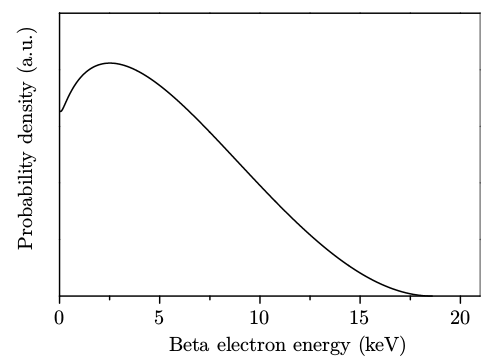
\includegraphics[scale=0.6]{Espectro.png}
\centering
\caption{\textbf{Figura 1}.-Espectro energético de los electrones de la desintegración del tritio ~\cite{TesisTritio}}
\end{figure}

Como era de esperar, este presenta la forma típica de un espectro energético de una desintegración $\beta$. Podemos observar que estos poseen una energía máxima de $18.6~\keV$, una energía promedio de $5.7~\keV$ y una moda (valor más probable) lígeramente inferior a la energía promedio, entorno a $4.5~\keV$. Con estos valores de energía podemos apreciar que la energía de radiación del tritio es la más pequeña observada hasta el momento en los isótopos. Como consecuencia el electrón presentará un recorrido libre medio muy corto, del orden de $3-5~\mm$ en el aire y de $5-6~\mu m$ en la fibra centelleadora.

El problema actual reside en que los mecanismos de detección y monitorización de tritio utilizados en la actualidad, en concreto en centrales nucleares, que será el objetivo final del detector que pretendemos desarrollar en el grupo experimental internacional denominado \textit{Tritium}, son métodos lentos o con un alto umbral de detección ~\cite{limiteMB}~\cite{Limitetiempo}~\cite{Limite}. 

Por ejemplo, entre los métodos más empleado actualmente en centrales nucleares, esta el método de detección de aguas tritiadas por medio de centelleo líquido. Este es el método más indicado para la detección de partículas beta de energía muy pequeña porque, como ya se ha visto al analizar el espectro energético de los electrones que conforman la radiación $\beta$ del tritio estos presentan un recorrido libre medio muy pequeño (del orden del mm o $\mu m$, dependiendo del medio (referencia)). Dado que solo contribuye a la medida (con una probabilidad aceptable) las emisiones que han tenido lugar a una distancia del detector inferior al recorrido libre medio la forma más efectiva de conseguir que un mayor volumen de la fuente radiactiva contribuya a la señal y que un mayor volumen del detector se encuentre a una distancia adecuada de la fuente radiactiva es disolviendo este detector con el líquido radiactivo (en nuestro caso agua tritiada), y esto solo se puede conseguir utilizando detectores líquidos de partículas beta, como el liquido centelleador. 

El método de centelleo líquido consiste en tomar una muestra del líquido radiactivo, agua tritiada en nuestro caso, diluirla (habitualmente al 50\%) con el líquido centelleador y medir los fotones emitidos por este líquido centelleador, a partir de los cuales podremos determinar los electrones emitidos por la muestra de agua tritiada y detectados por el líquido centelleador. Sin embargo para ello se necesita tomar una muestra y llevarla al laboratorio para el correspondiente estudio. En resumen se trata de un proceso de detección de agua tritiada basado en metodos offline que ralentizan la monitorización dilatando el resultado hasta varios dias desde la toma de la muestra. 

Tras cada análisis, la muestra de agua tritiada y líquido centelleador son inseparable y por tanto no reutilizable.  Este debe de ser tratado como residuo peligroso ya que, aunque el análisis desvele que el agua tritiada esta libre de tritio (presente una actividad suficientemente baja para ser tratada como material no radiactivo), esta contiene tolueno, presente en el líquido centelleador y, por tanto, debe de ser procesada de manera segura. También necesita operarios especializados manipulen estas muestras, poniendo en peligro su salud ~\cite{gel}.

El objetivo final de \textit{Tritium}, sobre el cual tratará mi futura tésis, es desarrollar un detector de aguas tritiadas que permita realizar la monitorización del tritio \textit{in situ} a tiempo real. Por tiempo real entendemos una dilatación temporal máxima de 10 minutos desde la toma de la muestra (ya que se necesita un tiempo mínimo para poder discernir la señal del background, el cual dependera, entre otras cosas, de la configuración del sistema de detección). Además el prototipo desarrollado no necesitará de la presencia de personal especializado que intervenga en el proceso de monitorización de aguas tritiadas, agilizando y abaratando el método de monitorización, además de excluir posibles errores humanos. El método simplemente requerirá continuas calibraciones al cabo de un tiempo determinado para asegurar el correcto funcionamiento del dispositivo. 

La dificultad aquí residirá en conseguir extraer esta señal tan pequeña ($\backsim\keV$) y tener estadística suficiente para poder discernirla del fondo radiactivo en un tiempo tan pequeño. Los trabajos \textit{in situ} con configuraciones del detector similares (centelleador + contador de fotones) realizados hasta la fecha que utilizan el concepto de tiempo real solo han conseguido obtener una señal en el límite del MeV ~\cite{TesisTritio}. Estos estan basados principalmente en solidos centelleadores y tubos fotomultiplicadores (PMT) a diferencia de nuestro experimento que consta de fibras centelleadoras (que detectan la radiación beta del tritio y la convierten en fotones) y tubos fotomultiplicadores o fotomultiplicadores de silicio (que detectan estos fotones y los convierten en electrones que conformarán la señal del sistema). 

En mi opinion el uso de fibras centelleadores es una mejor elección ya que presentan un mayor volumen activo con el que detectar el la radiación del tritio  sin necesidad de utilizar líquido centelleador el cual, como he mencionado anteriormente, produce residuos peligrosos además del coste del líquido centelleador no reutilizable. Además las fibras centelleadoras presentan un mayor abanico de posibilidades en cuanto a la elección de las distintas estructuras de las mismas. Nuestro experimento se centrará en la utilización de SiPM aunque también contemplará el uso de PMT. 

Hay que tener en cuenta que si existen diseños que logran llegar a límites del orden del Bequerelio en un tiempo de 3 minutos, aunque estos estan basados en configuraciones totalmente distintas, como por ejemplo un sistema, conformado por un láser y cavidades espectroscópicas en forma de anillo, en el cual se pretende buscar la existencia de resonacias y relacionar las frecuencias a las que estas ocurren con la concentración de tritio presente en la muestra. ~\cite{Anillo}. Sin embargo este es un estudio totalmente diferente ya que necesita de un acondicionamiento y control exhaustivo de las condiciones del sistema para el correcto funcionamiento del láser, encareciendo la construcción y mantenimiento del mismo y dificultando la existencia de este en sitios como centrales nucleares, es decir, es una aplicación que no persigue un mismo fín. 

Para conseguir extraer una señal tan pequeña con la mayor eficiencia posible estudiaremos diversas configuraciones experimentales para conseguir obtener la mas adecuada de acuerdo a nuestro objetivo experimental. Además realizaremos en todo momento detecciones en coincidencia, lo cual nos permitira eliminar en gran medida el fondo radiactivo del experimento. Las configuraciónes que pretendemos abarcar en el experimento son: 
\begin{itemize}
\item {}
Por un lado estudiaremos cual es la mejor elección para las estructuras de fibras centelleadores. Estudiaremos las ventajas y desventajas que presenta la utilización clads en las fibras (recubrimiento de la fibra centelleadora para evitar la fuga de fotones de centelleo y poder dirigir estos de manera opticamente aceptable hasta el contador de fotones). 
\item {}
Por otro lado estudiaremos cual es la mejor elección para un contador de fotones. Las posibilidades contempladas en el experimento serán SiPM o PMT. Veremos cual es más adecuado ya que cada una presenta una serie de características mejores como la eficiencia de fotodetección (PDE) de los SiPM sobre la de los PMT pero otras tantas peores como la dependencia con la temperatura más acusada en los SiPM que en los PMT.
\end{itemize}

También se realizarán una serie de simulaciones del experimento previas al desarrollo del mismo utilizando el programa "Geant 4", desarrollado por el cern, con el objetivo de ver que es el que deberíamos esperar teóricamente de nuestros resultados. Estas simulaciones nos permitiran comparar nuestros resultados experimentales con los datos simulados para ver hasta que punto nuestro experimento dista del modelo teórico seguido, lo cual nos permitira a su vez comprobar la fiabilidad de este modelo teórico y corregir posibles erratas del mismo. También nos permitirá ver que posibles modificaciones podemos realizar en el experimento para obtener un mejor resultado.

El grupo experimental \textit{Tritium} es un grupo internacional compuesto por tres paises: Portugal, Francia y España; En concreto intervienen las universidades de...  El proyecto que planteamos en este grupo es demasiado extenso para una trabajo de fín de master ya que se necesitan años para conseguir resultados concluyentes y, como ya se ha mencionado anteriormente, será la base de mi futura tésis. En este trabajo de fin de máser únicamente nos centraremos en los primeros pasos de este gran proyecto, el cual ha empezado recientemente y, afortunadamente, me ha permitido estar en este desde el inicio.

Dividiremos este trabajo en seis partes:
\begin{enumerate}
\item{} En primer lugar se realizará un pequeño estudio sobre las fibras centelleadoras. Por un lado se determinará cual es la forma adecuada de actuar a la hora de manipular fibras centelleadoras, elemento más sensible de los utilizados en el experimento, presentando el procedimiento final de como preparar un bunch de fibras centelleadoras con resultado opticamente aceptable. Por otro lado se utilizarán distintas estructuras de las mismas para ver cual nos permite obtener una señal del agua tritiada  más óptima. 

\item{} En segundo lugar realizaremos una calibración de los SiPM, paso fundamental antes de poder obtener cualquier medida del experimento. La finalidad de este paso es poder catalogar la magnitud de la medida del sistema que estamos obteniendo con este instrumento, algo fundamental en física. No se necesita realizar una calibración de los PMT, paso igualmente importante al anterior, ya que este trabajo fue realizado recientemente por otro componente del grupo.

\item{} En tercer lugar se describirá uno de las posibles configuraciones que serán estudiadas con el fin de determinar cual de estas es la más adecuada, desde el punto de vista del objetivo final de proyecto, para el diseño final del detector. Este también nos permitirá encontrar posibles fallos y mejoras que optimicen nuestro prototipo y que podrán ser utilizadas para el diseño final. En concreto la configuración que se estudiará esta formada por un bunch de 35 fibras centelleadoras sin clad leidas por PMT. También se hablará, entre otras cosas, del proceso de llenado que tuvo que ser desarrollado para una realización segura del mismo además del los resultados obtenidos.

\item{} En cuarto lugar se presentarán las simulaciones realizadas con el programa de Geant4, programa desarrollado por el cern capaz de realizar simulaciones muy detalladas de experimentos, principalmente de física de partículas. En este punto se presentaran las simulaciones realizadas tanto para los prototipos como para posibles diseños finales. Esto nos permitirá ver que posibles mejoras podemos incluir a nuestro experimento y en que puntos difieren los resultados obtenidos con las simulaciones con los resultados obtenidos en los distintos experimentos de los prototipo.

\item{} En quinto lugar se presentará se comentaran posibles partes del experimento que queden inconclusas o inacabadas o puntos interesantes y que serán propuestos a futuros estudios que habrá que realizar durante la tésis. También se comentará brevemente el siguiente paso que pretenderemos realizar en el proyecto.

\item{} Se presentará un último punto donde se expondrán las conclusiones alcanzadas durante la completitud del trabajo.

\end{enumerate}